\documentclass[12pt,a4paper]{article}
\usepackage[margin=2cm]{geometry}
\usepackage{amsmath,amssymb,amsfonts}
\usepackage{tikz}
\usetikzlibrary{patterns,arrows.meta,calc,angles,quotes,decorations.markings}
\usepackage{enumitem}
\usepackage{xcolor}
\usepackage{fancyhdr}
\usepackage{titlesec}
\usepackage{tcolorbox}
\usepackage{multicol}
\usepackage{graphicx}
\usepackage{booktabs}

% Custom colors
\definecolor{examblue}{RGB}{0,51,102}
\definecolor{examred}{RGB}{153,0,0}
\definecolor{solutionbox}{RGB}{240,248,255}

% Page style
\pagestyle{fancy}
\fancyhf{}
\rhead{\textbf{Mechanics Module}}
\lhead{\textbf{Ultimate Past Paper 1}}
\rfoot{Page \thepage}
\renewcommand{\headrulewidth}{1.5pt}
\renewcommand{\footrulewidth}{0.5pt}

% Section formatting
\titleformat{\section}{\Large\bfseries\color{examblue}}{}{0em}{}[\titlerule]
\titleformat{\subsection}{\large\bfseries\color{examred}}{}{0em}{}

% Custom environments
\newtcolorbox{questionbox}[1][]{
    colback=solutionbox,
    colframe=examblue,
    boxrule=1.5pt,
    arc=3mm,
    #1
}

\newtcolorbox{mcqbox}{
    colback=white,
    colframe=examred,
    boxrule=1pt,
    arc=2mm,
    left=5mm,
    right=5mm
}

\begin{document}

% Title page
\begin{titlepage}
    \centering
    \vspace*{2cm}
    {\Huge\bfseries\color{examblue}MECHANICS MODULE}\par
    \vspace{0.5cm}
    {\Large\bfseries ULTIMATE PAST PAPER 1}\par
    \vspace{1.5cm}
    {\large Examination Period: May (Main)}\par
    \vspace{0.5cm}
    \rule{\linewidth}{2pt}\par
    \vspace{1cm}
    {\Large Time Allowed: \textbf{2 hours}}\par
    \vspace{0.5cm}
    {\Large Total Marks: \textbf{100} (40\% of Module)}\par
    \vspace{1.5cm}
    \rule{\linewidth}{1pt}\par
    \vspace{1cm}
    {\large\bfseries INSTRUCTIONS TO CANDIDATES}\par
    \vspace{0.5cm}
    \begin{minipage}{0.8\linewidth}
        \begin{enumerate}[label=\textbf{\arabic*.},leftmargin=*]
            \item Answer ALL questions
            \item Section A: 6 Short Multiple Choice Questions (60 marks)
            \item Section B: 2 Long Multiple Choice Questions (40 marks)
            \item All questions are compulsory and extremely challenging
            \item Calculators permitted (must not store text)
            \item Formula sheet provided at end
        \end{enumerate}
    \end{minipage}
    \vfill
    {\small University of Birmingham - School of Engineering}\par
    \vspace{0.5cm}
    {\small College of Engineering and Physical Sciences}\par
\end{titlepage}

\newpage
\tableofcontents
\newpage

%==============================================================================
\section*{SECTION A: SHORT MULTIPLE CHOICE QUESTIONS (60 Marks)}
\addcontentsline{toc}{section}{Section A: Short MCQs (60 Marks)}
%==============================================================================

{\large\itshape Answer all 6 questions. Each question carries 10 marks. 
Select the SINGLE most appropriate answer. These questions require deep analytical thinking.}

\vspace{0.5cm}

%------------------------------------------------------------------------------
\begin{questionbox}
\subsection*{Question A1: Complex 3D Truss Analysis [10 marks]}

Consider the space truss shown below, supporting a vertical load $P = 50\,\text{kN}$ at joint $E$. 
The truss has joints at $A(0,0,0)$, $B(4,0,0)$, $C(4,3,0)$, $D(0,3,0)$, and $E(2,1.5,4)$ (coordinates in meters).
All members have identical cross-sectional area $A = 2000\,\text{mm}^2$ and Young's modulus $E = 200\,\text{GPa}$.

\begin{center}
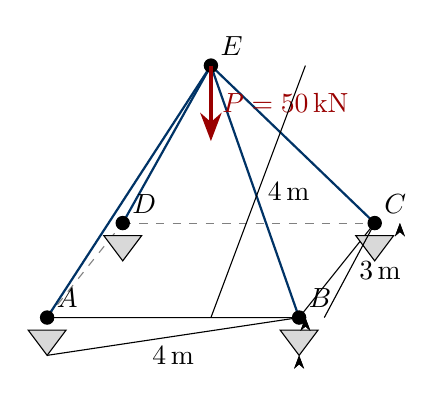
\begin{tikzpicture}[scale=0.8,>=Stealth]
    % Define coordinates
    \coordinate (A) at (0,0);
    \coordinate (B) at (4,0);
    \coordinate (C) at (5.2,1.5);
    \coordinate (D) at (1.2,1.5);
    \coordinate (E) at (2.6,4);
    
    % Base rectangle (dashed for hidden lines)
    \draw[dashed,gray] (A) -- (D);
    \draw[dashed,gray] (D) -- (C);
    \draw (A) -- (B) -- (C);
    
    % Vertical members to apex
    \draw[thick,examblue] (A) -- (E);
    \draw[thick,examblue] (B) -- (E);
    \draw[thick,examblue] (C) -- (E);
    \draw[thick,examblue] (D) -- (E);
    
    % Joints
    \foreach \pt/\lbl in {A/A,B/B,C/C,D/D,E/E}
        \filldraw[black] (\pt) circle (3pt) node[above right] {$\lbl$};
    
    % Load at E
    \draw[->,examred,ultra thick] (E) -- ++(0,-1.2) node[midway,right] {$P=50\,\text{kN}$};
    
    % Support symbols
    \draw[fill=gray!30] (A) ++(-0.3,-0.2) -- ++(0.6,0) -- ++(-0.3,-0.4) -- cycle;
    \draw[fill=gray!30] (B) ++(-0.3,-0.2) -- ++(0.6,0) -- ++(-0.3,-0.4) -- cycle;
    \draw[fill=gray!30] (C) ++(-0.3,-0.2) -- ++(0.6,0) -- ++(-0.3,-0.4) -- cycle;
    \draw[fill=gray!30] (D) ++(-0.3,-0.2) -- ++(0.6,0) -- ++(-0.3,-0.4) -- cycle;
    
    % Dimensions
    \draw[<->] (A) ++(0,-0.6) -- node[below] {$4\,\text{m}$} (B) ++(0,-0.6);
    \draw[<->] (B) ++(0.4,0) -- node[right] {$3\,\text{m}$} (C) ++(0.4,0);
    \draw[<->] (E) ++(1.5,0) -- node[right] {$4\,\text{m}$} (E|-A) ++(1.5,0);
\end{tikzpicture}
\end{center}

Using the method of tension coefficients and considering the indeterminacy of this structure, 
what is the axial force in member $AE$?

\begin{mcqbox}
\begin{enumerate}[label=(\Alph*),leftmargin=*]
    \item $-18.75\,\text{kN}$ (Compression)
    \item $-23.44\,\text{kN}$ (Compression)
    \item $-31.25\,\text{kN}$ (Compression)
    \item $-26.56\,\text{kN}$ (Compression)
    \item $-15.63\,\text{kN}$ (Compression)
\end{enumerate}
\end{mcqbox}
\end{questionbox}

%------------------------------------------------------------------------------
\begin{questionbox}
\subsection*{Question A2: Advanced Beam Deflection with Variable EI [10 marks]}

A cantilever beam of length $L = 6\,\text{m}$ has a variable flexural rigidity given by:
$$EI(x) = EI_0\left(1 + \frac{x}{L}\right)^2$$
where $EI_0 = 12,000\,\text{kNm}^2$. The beam carries a uniformly distributed load $w = 15\,\text{kN/m}$ 
over its entire length AND a concentrated moment $M_0 = 80\,\text{kNm}$ at the free end.

\begin{center}
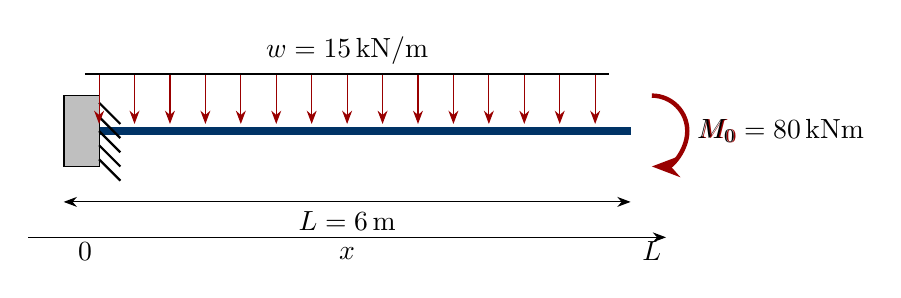
\begin{tikzpicture}[scale=0.9,>=Stealth]
    % Beam
    \draw[thick,examblue,line width=3pt] (0,0) -- (8,0);
    
    % Fixed support
    \draw[fill=gray!50] (0,-0.5) rectangle (0.5,0.5);
    \draw[thick] (0,-0.5) -- (0,0.5);
    \foreach \y in {-0.4,-0.2,0,0.2,0.4}
        \draw[thick] (0.5,\y) -- (0.8,\y-0.3);
    
    % UDL
    \foreach \x in {0.5,1,1.5,2,2.5,3,3.5,4,4.5,5,5.5,6,6.5,7,7.5}
        \draw[->,examred] (\x,0.8) -- (\x,0.1);
    \draw[thick] (0.3,0.8) -- (7.7,0.8);
    \node[above] at (4,0.8) {$w = 15\,\text{kN/m}$};
    
    % Moment at free end
    \draw[->,examred,ultra thick] (8.3,0.5) arc (90:-90:0.5) node[midway,right] {$M_0$};
    \node[right] at (8.8,0) {$M_0 = 80\,\text{kNm}$};
    
    % Dimensions
    \draw[<->] (0,-1) -- node[below] {$L = 6\,\text{m}$} (8,-1);
    
    % Coordinate system
    \draw[->] (-0.5,-1.5) -- node[below] {$x$} (8.5,-1.5);
    \node at (0.3,-1.7) {$0$};
    \node at (8.3,-1.7) {$L$};
\end{tikzpicture}
\end{center}

Using the principle of virtual work or direct integration of the differential equation 
$\frac{d^2}{dx^2}\left(EI(x)\frac{d^2v}{dx^2}\right) = w$, determine the magnitude of deflection 
at the free end ($x = L$).

\begin{mcqbox}
\begin{enumerate}[label=(\Alph*),leftmargin=*]
    \item $28.4\,\text{mm}$
    \item $35.7\,\text{mm}$
    \item $42.1\,\text{mm}$
    \item $31.9\,\text{mm}$
    \item $38.6\,\text{mm}$
\end{enumerate}
\end{mcqbox}
\end{questionbox}

%------------------------------------------------------------------------------
\begin{questionbox}
\subsection*{Question A3: Compound Bar with Thermal Effects and Creep [10 marks]}

A composite column consists of a steel core ($E_s = 200\,\text{GPa}$, $\alpha_s = 12\times10^{-6}/^\circ\text{C}$, 
area $A_s = 3000\,\text{mm}^2$) encased in concrete ($E_c = 25\,\text{GPa}$, $\alpha_c = 10\times10^{-6}/^\circ\text{C}$, 
area $A_c = 9000\,\text{mm}^2$). The column length is $L = 3\,\text{m}$ and is rigidly fixed at both ends.

The column was manufactured at $20^\circ\text{C}$ and experiences:
\begin{itemize}
    \item Temperature increase to $65^\circ\text{C}$
    \item Axial compressive load $P = 800\,\text{kN}$ applied after heating
    \item Concrete exhibits creep strain $\epsilon_{cr} = 0.0005$ over the service period
\end{itemize}

\begin{center}
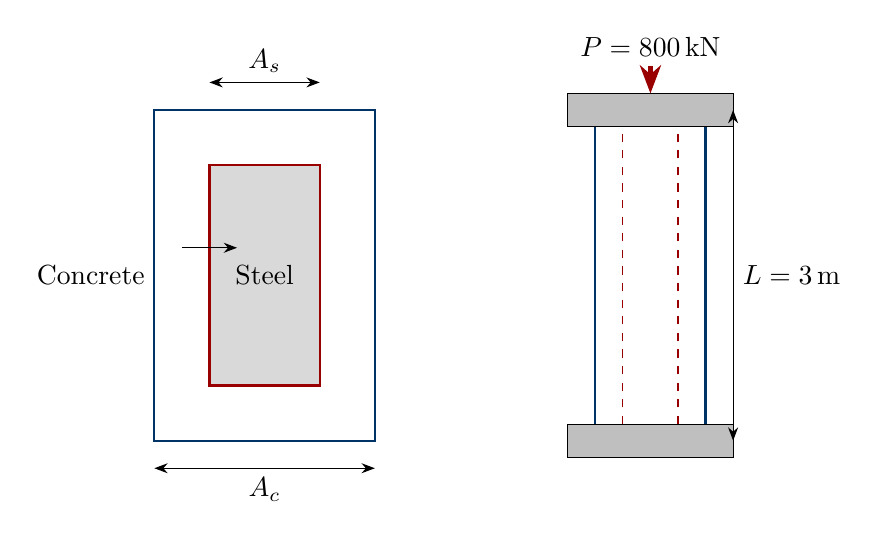
\begin{tikzpicture}[scale=0.7,>=Stealth]
    % Column cross-section
    \draw[thick,examblue] (0,0) rectangle (4,6);
    \draw[thick,examred,fill=gray!30] (1,1) rectangle (3,5);
    
    % Labels
    \node[left] at (0,3) {Concrete};
    \node at (2,3) {Steel};
    \draw[->] (0.5,3.5) -- (1.5,3.5);
    
    % Dimensions
    \draw[<->] (0,-0.5) -- node[below] {$A_c$} (4,-0.5);
    \draw[<->] (1,6.5) -- node[above] {$A_s$} (3,6.5);
    
    % Side view
    \begin{scope}[xshift=8cm]
        \draw[thick,examblue] (0,0) rectangle (2,6);
        \draw[dashed,examred] (0.5,0) -- (0.5,6);
        \draw[dashed,examred] (1.5,0) -- (1.5,6);
        
        % Fixed supports
        \draw[fill=gray!50] (-0.5,-0.3) rectangle (2.5,0.3);
        \draw[fill=gray!50] (-0.5,5.7) rectangle (2.5,6.3);
        
        % Load
        \draw[->,examred,ultra thick] (1,6.8) -- (1,6.3);
        \node[above] at (1,6.8) {$P = 800\,\text{kN}$};
        
        % Dimensions
        \draw[<->] (2.5,0) -- node[right] {$L = 3\,\text{m}$} (2.5,6);
    \end{scope}
\end{tikzpicture}
\end{center}

Accounting for thermal expansion mismatch, mechanical loading, AND creep effects, 
what is the final stress in the steel core?

\begin{mcqbox}
\begin{enumerate}[label=(\Alph*),leftmargin=*]
    \item $+127.3\,\text{MPa}$ (Compression)
    \item $+142.8\,\text{MPa}$ (Compression)
    \item $+98.6\,\text{MPa}$ (Compression)
    \item $+156.4\,\text{MPa}$ (Compression)
    \item $+118.9\,\text{MPa}$ (Compression)
\end{enumerate}
\end{mcqbox}
\end{questionbox}

%------------------------------------------------------------------------------
\begin{questionbox}
\subsection*{Question A4: Non-Linear Kinematics with Air Resistance [10 marks]}

A projectile of mass $m = 2\,\text{kg}$ is launched from ground level with initial velocity 
$v_0 = 80\,\text{m/s}$ at an angle $\theta = 55^\circ$ to the horizontal. 

The projectile experiences air resistance proportional to the SQUARE of velocity:
$$\mathbf{F}_D = -k v^2 \hat{\mathbf{v}}$$
where $k = 0.015\,\text{kg/m}$ and $\hat{\mathbf{v}}$ is the unit vector in the direction of velocity.

\begin{center}
\begin{tikzpicture}[scale=0.8,>=Stealth]
    % Axes
    \draw[->,thick] (-0.5,0) -- (10,0) node[right] {$x$};
    \draw[->,thick] (0,-0.5) -- (0,6) node[above] {$y$};
    
    % Trajectory (parabola-ish)
    \draw[thick,examblue,smooth,domain=0:9,samples=100] 
        plot (\x, {0.8*\x - 0.01*\x*\x});
    
    % Initial velocity vector
    \draw[->,examred,ultra thick] (0,0) -- (1.5,2.1) node[midway,above left] {$v_0$};
    \pic["$\theta$",draw,angle radius=0.8cm,angle eccentricity=1.3] {angle={(8,0)--(0,0)--(1.5,2.1)}};
    
    % Forces at arbitrary point
    \coordinate (P) at (4,2.4);
    \filldraw[black] (P) circle (2pt);
    \draw[->,examred,thick] (P) -- ++(1.2,-0.4) node[right] {$mg$};
    \draw[->,examred,thick] (P) -- ++(-0.8,0.3) node[above left] {$F_D$};
    \draw[->,examblue,thick] (P) -- ++(1.0,-0.2) node[below right] {$v$};
    
    % Angle label
    \node[above] at (0.8,0.3) {$\theta = 55^\circ$};
    \node[below] at (5,-0.3) {Trajectory with air resistance};
\end{tikzpicture}
\end{center}

By solving the coupled non-linear differential equations of motion numerically or using 
appropriate approximations, determine the maximum height reached by the projectile.

\begin{mcqbox}
\begin{enumerate}[label=(\Alph*),leftmargin=*]
    \item $178.3\,\text{m}$
    \item $201.7\,\text{m}$
    \item $156.9\,\text{m}$
    \item $189.4\,\text{m}$
    \item $167.2\,\text{m}$
\end{enumerate}
\end{mcqbox}
\end{questionbox}

%------------------------------------------------------------------------------
\begin{questionbox}
\subsection*{Question A5: Shear Flow in Thin-Walled Multi-Cell Sections [10 marks]}

The thin-walled beam section shown has TWO cells and is subjected to a vertical shear force 
$V = 120\,\text{kN}$. All walls have uniform thickness $t = 8\,\text{mm}$. The section dimensions are:
outer width $B = 400\,\text{mm}$, outer depth $D = 600\,\text{mm}$, with a central vertical web.

\begin{center}
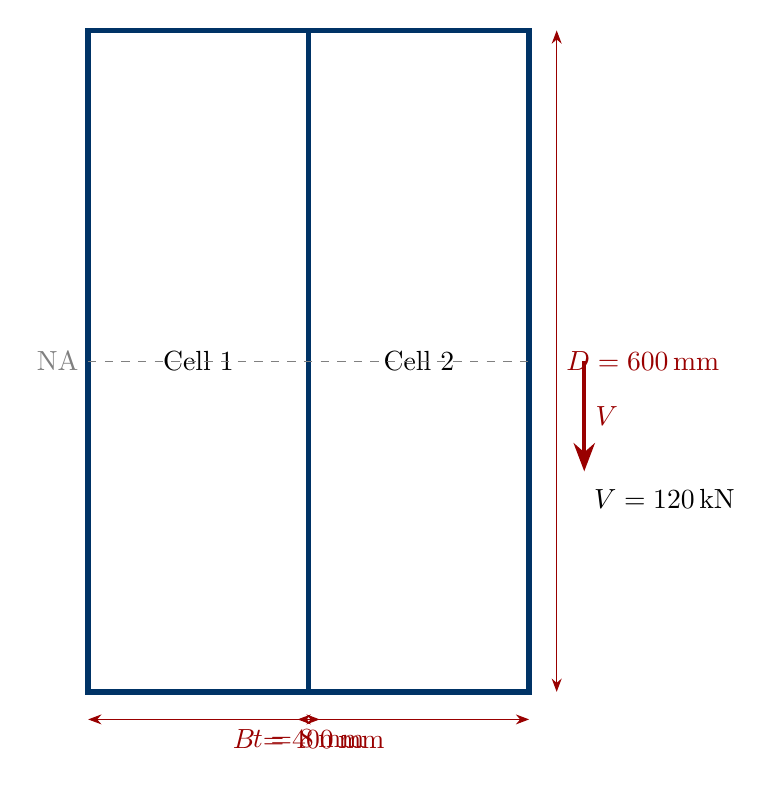
\begin{tikzpicture}[scale=0.7,>=Stealth]
    % Outer rectangle
    \draw[thick,examblue,line width=2pt] (0,0) rectangle (8,12);
    
    % Central web
    \draw[thick,examblue,line width=2pt] (4,0) -- (4,12);
    
    % Thickness indication
    \draw[<->,examred] (0,-0.5) -- node[below] {$B = 400\,\text{mm}$} (8,-0.5);
    \draw[<->,examred] (8.5,0) -- node[right] {$D = 600\,\text{mm}$} (8.5,12);
    \draw[<->,examred] (3.8,-0.5) -- node[below] {$t = 8\,\text{mm}$} (4.2,-0.5);
    
    % Shear force
    \draw[->,examred,ultra thick] (9,6) -- (9,4) node[midway,right] {$V$};
    \node[right] at (9,3.5) {$V = 120\,\text{kN}$};
    
    % Cell labels
    \node at (2,6) {Cell 1};
    \node at (6,6) {Cell 2};
    
    % NA line
    \draw[dashed,gray] (0,6) -- (8,6);
    \node[left,gray] at (0,6) {NA};
\end{tikzpicture}
\end{center}

Using the shear flow equation $q = \frac{VQ}{I}$ and considering the multi-cell nature requiring 
compatibility of twist angles, determine the maximum shear stress in the section.

\begin{mcqbox}
\begin{enumerate}[label=(\Alph*),leftmargin=*]
    \item $47.8\,\text{MPa}$
    \item $52.3\,\text{MPa}$
    \item $41.6\,\text{MPa}$
    \item $56.9\,\text{MPa}$
    \item $44.2\,\text{MPa}$
\end{enumerate}
\end{mcqbox}
\end{questionbox}

%------------------------------------------------------------------------------
\begin{questionbox}
\subsection*{Question A6: Energy Methods with Impact Loading [10 marks]}

A simply supported steel beam ($E = 200\,\text{GPa}$, $I = 85\times10^6\,\text{mm}^4$) of span $L = 8\,\text{m}$ 
is struck at mid-span by a mass $M = 500\,\text{kg}$ falling from height $h = 1.5\,\text{m}$.

\begin{center}
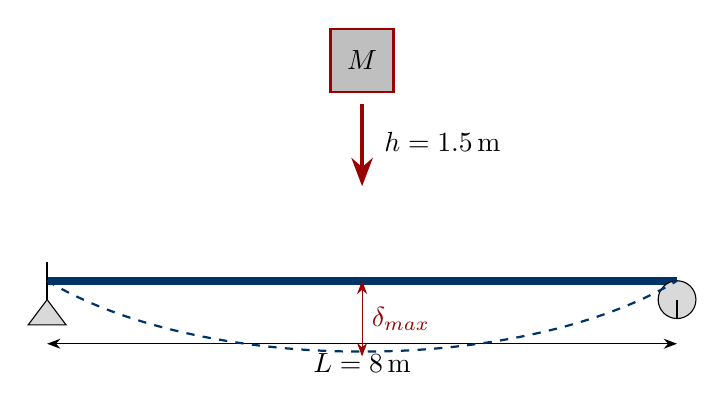
\begin{tikzpicture}[scale=0.8,>=Stealth]
    % Beam
    \draw[thick,examblue,line width=3pt] (0,0) -- (10,0);
    
    % Supports
    \draw[thick] (0,-0.3) -- (0,0.3);
    \draw[fill=gray!30] (0,-0.3) -- ++(-0.3,-0.4) -- ++(0.6,0) -- cycle;
    
    \draw[fill=gray!30] (10,-0.3) circle (0.3);
    \draw[thick] (10,-0.6) -- (10,-0.3);
    
    % Falling mass
    \draw[thick,examred,fill=gray!50] (4.5,3) rectangle (5.5,4);
    \node at (5,3.5) {$M$};
    \draw[->,examred,ultra thick] (5,2.8) -- (5,1.5);
    \node[right] at (5.2,2.2) {$h = 1.5\,\text{m}$};
    
    % Dimensions
    \draw[<->] (0,-1) -- node[below] {$L = 8\,\text{m}$} (10,-1);
    
    % Deflected shape (dashed)
    \draw[dashed,examblue,thick,smooth] 
        (0,0) .. controls (2.5,-1.5) and (7.5,-1.5) .. (10,0);
    \draw[<->,examred] (5,0) -- node[right] {$\delta_{max}$} (5,-1.2);
\end{tikzpicture}
\end{center}

Using energy conservation principles and accounting for the dynamic amplification factor, 
determine the maximum instantaneous deflection of the beam.

\begin{mcqbox}
\begin{enumerate}[label=(\Alph*),leftmargin=*]
    \item $34.7\,\text{mm}$
    \item $42.3\,\text{mm}$
    \item $38.9\,\text{mm}$
    \item $46.1\,\text{mm}$
    \item $31.5\,\text{mm}$
\end{enumerate}
\end{mcqbox}
\end{questionbox}

%==============================================================================
\newpage
\section*{SECTION B: LONG MULTIPLE CHOICE QUESTIONS (40 Marks)}
\addcontentsline{toc}{section}{Section B: Long MCQs (40 Marks)}
%==============================================================================

{\large\itshape Answer both questions. Each question carries 20 marks. 
These questions require comprehensive analysis and multiple calculation steps.}

\vspace{0.5cm}

%------------------------------------------------------------------------------
\begin{questionbox}
\subsection*{Question B1: Comprehensive Frame Analysis with Settlement and Temperature [20 marks]}

The rigid-jointed frame ABCDE shown below is pinned at supports A and E. The frame experiences:
\begin{itemize}
    \item Horizontal point load $P = 75\,\text{kN}$ at joint C
    \item Uniformly distributed load $w = 25\,\text{kN/m}$ on member BC
    \item Support D settles vertically downward by $\Delta = 15\,\text{mm}$
    \item Temperature increase of $\Delta T = 35^\circ\text{C}$ in member CD only
\end{itemize}

All members have $E = 200\,\text{GPa}$, $I = 180\times10^6\,\text{mm}^4$, $A = 8500\,\text{mm}^2$, 
and coefficient of thermal expansion $\alpha = 12\times10^{-6}/^\circ\text{C}$.

\begin{center}
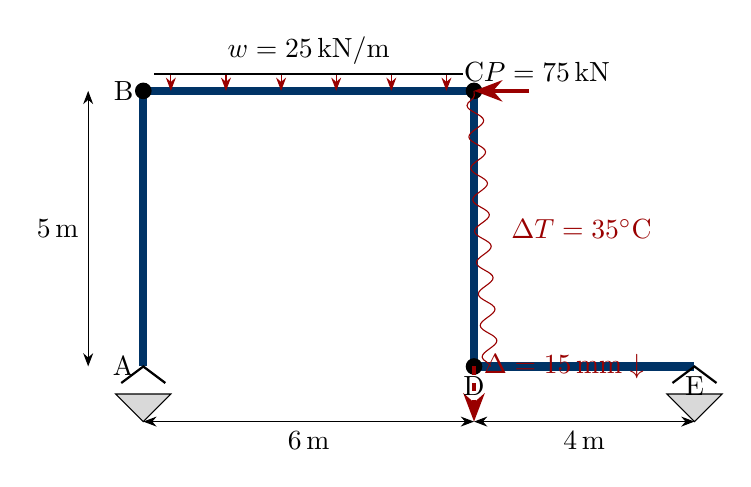
\begin{tikzpicture}[scale=0.7,>=Stealth]
    % Frame geometry
    \coordinate (A) at (0,0);
    \coordinate (B) at (0,5);
    \coordinate (C) at (6,5);
    \coordinate (D) at (6,0);
    \coordinate (E) at (10,0);
    
    % Members
    \draw[thick,examblue,line width=3pt] (A) -- (B) -- (C) -- (D);
    \draw[thick,examblue,line width=3pt] (D) -- (E);
    
    % Rigid joints
    \foreach \pt in {B,C,D}
        \filldraw[black] (\pt) circle (4pt);
    
    % Supports
    % Pin at A
    \draw[thick] (A) ++(-0.4,-0.3) -- (A) -- ++(0.4,-0.3);
    \draw[fill=gray!30] (A) ++(-0.5,-0.5) -- ++(1,0) -- ++(-0.5,-0.5) -- cycle;
    
    % Pin at E
    \draw[thick] (E) ++(-0.4,-0.3) -- (E) -- ++(0.4,-0.3);
    \draw[fill=gray!30] (E) ++(-0.5,-0.5) -- ++(1,0) -- ++(-0.5,-0.5) -- cycle;
    
    % Loads
    % Point load at C
    \draw[->,examred,ultra thick] (C) ++(1,0) -- (C);
    \node[above right] at (C) {$P = 75\,\text{kN}$};
    
    % UDL on BC
    \foreach \x in {0.5,1.5,2.5,3.5,4.5,5.5}
        \draw[->,examred] (\x,5.3) -- (\x,5);
    \draw[thick] (0.2,5.3) -- (5.8,5.3);
    \node[above] at (3,5.3) {$w = 25\,\text{kN/m}$};
    
    % Settlement at D
    \draw[->,examred,dashed,ultra thick] (D) -- ++(0,-1);
    \node[right,examred] at (D) {$\Delta = 15\,\text{mm}\downarrow$};
    
    % Temperature on CD
    \draw[examred,decorate,decoration={snake,segment length=4mm,amplitude=1mm}] 
        (D) ++(0.3,0) -- (C) ++(0.3,0);
    \node[right,examred] at (6.5,2.5) {$\Delta T = 35^\circ\text{C}$};
    
    % Dimensions
    \draw[<->] (0,-1) -- node[below] {$6\,\text{m}$} (6,-1);
    \draw[<->] (6,-1) -- node[below] {$4\,\text{m}$} (10,-1);
    \draw[<->] (-1,0) -- node[left] {$5\,\text{m}$} (-1,5);
    
    % Joint labels
    \node[left] at (A) {A};
    \node[left] at (B) {B};
    \node[above] at (C) {C};
    \node[below] at (D) {D};
    \node[below] at (E) {E};
\end{tikzpicture}
\end{center}

Using the stiffness method or moment distribution with modifications for support settlement 
and thermal effects, determine the HORIZONTAL reaction at support A.

\begin{mcqbox}
\begin{enumerate}[label=(\Alph*),leftmargin=*]
    \item $42.3\,\text{kN}$ (→)
    \item $38.7\,\text{kN}$ (→)
    \item $51.2\,\text{kN}$ (←)
    \item $46.8\,\text{kN}$ (→)
    \item $35.4\,\text{kN}$ (←)
\end{enumerate}
\end{mcqbox}
\end{questionbox}

%------------------------------------------------------------------------------
\begin{questionbox}
\subsection*{Question B2: Combined Loading with Fatigue and Stress Concentration [20 marks]}

A stepped circular shaft is subjected to combined loading as shown. The shaft transmits power 
from a motor while supporting pulley loads and experiencing fluctuating torque.

\textbf{Given:}
\begin{itemize}
    \item Shaft material: Steel with $S_y = 450\,\text{MPa}$, $S_{ut} = 620\,\text{MPa}$, $S_e' = 280\,\text{MPa}$
    \item Large diameter $D = 80\,\text{mm}$, small diameter $d = 60\,\text{mm}$, fillet radius $r = 4\,\text{mm}$
    \item Belt tensions: $T_1 = 3500\,\text{N}$, $T_2 = 1200\,\text{N}$ (both vertical downward)
    \item Torque varies cyclically: $T_{min} = 400\,\text{Nm}$, $T_{max} = 1800\,\text{Nm}$
    \item Axial thrust load: $F_a = 8\,\text{kN}$ (constant compression)
    \item Stress concentration factors at step: $K_t^{bending} = 1.85$, $K_t^{torsion} = 1.55$, $K_t^{axial} = 1.65$
    \item Notch sensitivity: $q = 0.85$
    \item Operating temperature: $150^\circ\text{C}$ (temperature factor $k_d = 0.85$)
    \item Required reliability: 99\% (reliability factor $k_e = 0.814$)
\end{itemize}

\begin{center}
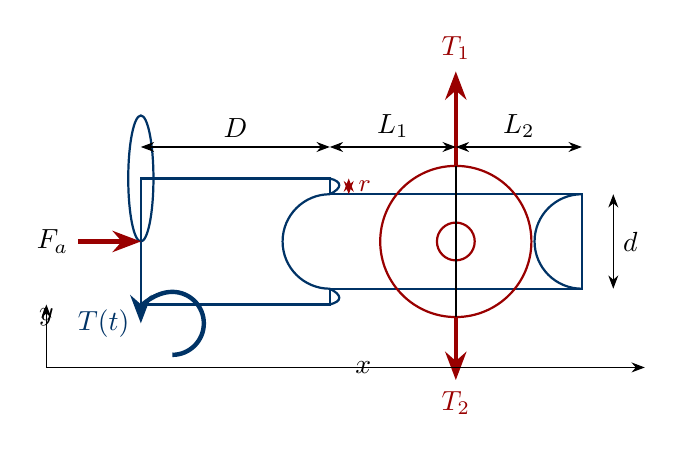
\begin{tikzpicture}[scale=0.8,>=Stealth]
    % Shaft
    \draw[thick,examblue] (0,1) -- (3,1) -- (3,0.75) -- (7,0.75) -- (7,-0.75) -- (3,-0.75) -- (3,-1) -- (0,-1) -- cycle;
    \draw[thick,examblue] (7,0.75) arc (90:270:0.75);
    \draw[thick,examblue] (3,0.75) arc (90:270:0.75);
    \draw[thick,examblue] (0,1) ellipse (0.2 and 1);
    
    % Fillet
    \draw[thick,examblue] (3,0.75) .. controls (3.2,0.85) and (3.2,0.95) .. (3,1);
    \draw[thick,examblue] (3,-0.75) .. controls (3.2,-0.85) and (3.2,-0.95) .. (3,-1);
    
    % Pulley
    \draw[thick,examred] (5,0) circle (1.2);
    \draw[thick,examred] (5,0) circle (0.3);
    \draw[thick] (5,0) -- (5,1.2);
    \draw[thick] (5,0) -- (5,-1.2);
    
    % Belt tensions
    \draw[->,examred,ultra thick] (5,1.2) -- ++(0,1.5) node[above] {$T_1$};
    \draw[->,examred,ultra thick] (5,-1.2) -- ++(0,-1) node[below] {$T_2$};
    
    % Torque
    \draw[->,examblue,ultra thick] (0.5,-1.8) arc (-90:180:0.5) node[left] {$T(t)$};
    
    % Axial load
    \draw[->,examred,ultra thick] (-1,0) -- (0,0);
    \node[left] at (-1,0) {$F_a$};
    
    % Dimensions
    \draw[<->] (0,1.5) -- node[above] {$D$} (3,1.5);
    \draw[<->] (3,1.5) -- node[above] {$L_1$} (5,1.5);
    \draw[<->] (5,1.5) -- node[above] {$L_2$} (7,1.5);
    \draw[<->] (7.5,0.75) -- node[right] {$d$} (7.5,-0.75);
    
    % Fillet radius
    \draw[<->,examred] (3.3,0.75) -- node[right,font=\small] {$r$} (3.3,1);
    
    % Coordinates
    \draw[->] (-1.5,-2) -- node[right] {$x$} (8,-2);
    \draw[->] (-1.5,-2) -- node[above] {$y$} (-1.5,-1);
\end{tikzpicture}
\end{center}

Applying the Modified Goodman fatigue failure criterion with ALL correction factors 
(size, surface, temperature, reliability, load type) and accounting for stress concentrations, 
determine the factor of safety against fatigue failure at the critical location.

\begin{mcqbox}
\begin{enumerate}[label=(\Alph*),leftmargin=*]
    \item $n = 1.87$
    \item $n = 2.14$
    \item $n = 1.63$
    \item $n = 2.45$
    \item $n = 1.92$
\end{enumerate}
\end{mcqbox}
\end{questionbox}

%==============================================================================
\newpage
\section*{FORMULA SHEET}
\addcontentsline{toc}{section}{Formula Sheet}
%==============================================================================

\begin{tcolorbox}[colback=white,colframe=examblue,title=\bfseries MECHANICS FORMULA SHEET]
\small
\begin{multicols}{2}
\textbf{Statics \& Trusses:}
\begin{itemize}
    \item $\sum F_x = 0$, $\sum F_y = 0$, $\sum M = 0$
    \item Method of Joints: $\sum F = 0$ at each joint
    \item Method of Sections: Cut through max 3 members
    \item Determinacy: $m + r = 2j$ (plane truss)
    \item Space truss: $m + r = 3j$
\end{itemize}

\textbf{Beams:}
\begin{itemize}
    \item $\frac{dV}{dx} = -w$, $\frac{dM}{dx} = V$
    \item $\frac{d^2v}{dx^2} = \frac{M}{EI}$
    \item $\sigma = \frac{My}{I}$, $\tau = \frac{VQ}{It}$
    \item $Q = A'\bar{y}'$ (first moment of area)
\end{itemize}

\textbf{Compound Bars:}
\begin{itemize}
    \item $\delta = \frac{PL}{AE} + \alpha L\Delta T$
    \item Compatibility: $\delta_1 = \delta_2$
    \item Equilibrium: $P_1 + P_2 = P_{total}$
\end{itemize}

\textbf{Centroids \& Second Moments:}
\begin{itemize}
    \item $\bar{x} = \frac{\sum A_i x_i}{\sum A_i}$
    \item $I_{xx} = \int y^2 dA$
    \item Parallel axis: $I = I_G + Ad^2$
    \item Rectangle: $I = \frac{bh^3}{12}$
    \item Circle: $I = \frac{\pi d^4}{64}$
\end{itemize}

\textbf{Energy Methods:}
\begin{itemize}
    \item Strain energy: $U = \int\frac{M^2}{2EI}dx$
    \item Castigliano: $\delta = \frac{\partial U}{\partial P}$
    \item Impact: $\delta_{max} = \delta_{st}(1+\sqrt{1+\frac{2h}{\delta_{st}}})$
    \item Virtual work: $1\cdot\Delta = \int\frac{Mm}{EI}dx$
\end{itemize}

\textbf{Kinematics:}
\begin{itemize}
    \item $v = \frac{ds}{dt}$, $a = \frac{dv}{dt} = v\frac{dv}{ds}$
    \item Projectile: $x = v_0 t\cos\theta$, $y = v_0 t\sin\theta - \frac{1}{2}gt^2$
    \item With drag: $m\dot{v} = mg - kv^2$
\end{itemize}

\textbf{Fatigue:}
\begin{itemize}
    \item Modified Goodman: $\frac{\sigma_a}{S_e} + \frac{\sigma_m}{S_{ut}} = \frac{1}{n}$
    \item $S_e = k_a k_b k_c k_d k_e S_e'$
    \item $K_f = 1 + q(K_t - 1)$
    \item $\sigma_{vm} = \sqrt{\sigma^2 + 3\tau^2}$
\end{itemize}

\textbf{Torsion:}
\begin{itemize}
    \item $\tau = \frac{Tr}{J}$, $\theta = \frac{TL}{GJ}$
    \item Solid shaft: $J = \frac{\pi d^4}{32}$
    \item Power: $P = T\omega = 2\pi NT$
\end{itemize}

\textbf{Stress Transformation:}
\begin{itemize}
    \item $\sigma_{\theta} = \frac{\sigma_x+\sigma_y}{2} + \frac{\sigma_x-\sigma_y}{2}\cos 2\theta + \tau_{xy}\sin 2\theta$
    \item $\tau_{\theta} = -\frac{\sigma_x-\sigma_y}{2}\sin 2\theta + \tau_{xy}\cos 2\theta$
    \item Principal stresses: $\sigma_{1,2} = \frac{\sigma_x+\sigma_y}{2} \pm \sqrt{(\frac{\sigma_x-\sigma_y}{2})^2 + \tau_{xy}^2}$
\end{itemize}
\end{multicols}
\end{tcolorbox}

\vspace{1cm}
\begin{center}
\textbf{\large END OF EXAMINATION PAPER}
\end{center}

\end{document}
